\documentclass[UTF8]{ctexart} % 文档类型中文tex

% 设置页边距
\usepackage{geometry}
\geometry{a4paper,scale=0.9}

% 显示代码和结果
\usepackage{codeshow}

% tikz
\usepackage{tikz}
\usetikzlibrary{positioning}

% 文档信息
\title{tikz 画图}
\date{\today}

\begin{document}

  \maketitle

  \section{简单图形}
  \subsection{直线}

  \begin{codeshow}
  \begin{tikzpicture}
    \draw (1,0) -- (0,0) -- (0,1);
  \end{tikzpicture}
  \end{codeshow}

  \begin{codeshow}
  \begin{tikzpicture}
    \draw (-1.5,0) -- (1.5,0);
    \draw (0,-1.5) -- (0,1.5);
  \end{tikzpicture}
  \end{codeshow}

\subsection{绘制曲线}

\begin{codeshow}
  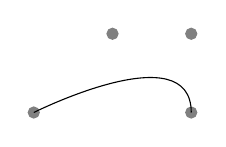
\begin{tikzpicture}
    \filldraw[gray] (0,0) circle [radius=2pt]
                    (1,1) circle [radius=2pt]
                    (2,1) circle [radius=2pt]
                    (2,0) circle [radius=2pt];
    \draw (0,0) .. controls (0,0) and (2,1) .. (2,0);

  \end{tikzpicture}
\end{codeshow}

可以通过这种方式画圆:
\begin{codeshow}
  \begin{tikzpicture}
    \draw (-1.5,0) -- (1.5,0);
    \draw (0,-1.5) -- (0,1.5);
    \draw (-1,0) .. controls (-1,0.555) and (-0.555,1) .. (0,1)
                 .. controls (0.555,1) and (1,0.555) ..(1,0);
  \end{tikzpicture}
\end{codeshow}

\subsection{绘制圆形}

\begin{codeshow}
  \tikz \draw (0,0) circle [radius=10pt];
\end{codeshow}

椭圆
\begin{codeshow}
  \tikz \draw (0,0) ellipse [x radius=10pt, y radius=5pt];
\end{codeshow}

接下来可以这样画圆形
\begin{codeshow}
  \begin{tikzpicture}
    \draw (-1.5,0) -- (1.5,0);
    \draw (0,-1.5) -- (0,1.5);
    \draw (0,0) circle [radius=1cm];
  \end{tikzpicture}
\end{codeshow}

\subsection{方形}
\begin{codeshow}
  \tikz \draw (-0.5,-0.5) rectangle (-1,-1);
\end{codeshow}

\subsection{绘制网格}
\begin{codeshow}
  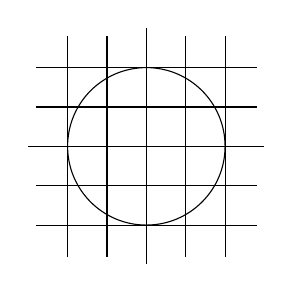
\begin{tikzpicture}
    \draw (-1.5,0) -- (1.5,0);
    \draw (0,-1.5) -- (0,1.5);
    \draw (0,0) circle [radius=1cm];
    \draw[step=.5cm] (-1.4,-1.4) grid (1.4, 1.4);
  \end{tikzpicture}
\end{codeshow}
然后将网格美化成灰色
\begin{codeshow}
  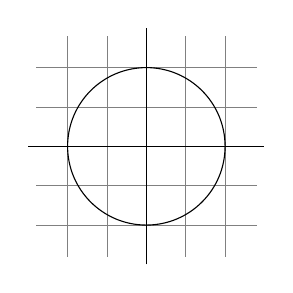
\begin{tikzpicture}
    \draw[step=.5cm, gray, very thin] (-1.4,-1.4) grid (1.4, 1.4);
    \draw (-1.5,0) -- (1.5,0);
    \draw (0,-1.5) -- (0,1.5);
    \draw (0,0) circle [radius=1cm];
  \end{tikzpicture}
\end{codeshow}
\end{document}
